\documentclass[10pt,a4paper]{article}
\usepackage[utf8]{inputenc}
\usepackage{amsmath}
\usepackage{amsthm}
\usepackage{amsfonts}
\usepackage{amssymb}
\usepackage{geometry}
\usepackage{graphicx}
\author{Nicolò Fornari}
\title{Network security}
\newtheorem{remark}{Remark}
\begin{document}
\maketitle
\section{Network protocols}
\textbf{Data link layer}\\
It is the lowest logical level, the data link interconnects physical interfaces. Each interface is identified by a MAC address (Media Access Control).\\
The MAC address is 48 bit long, it is usually represented in Hex notation and it is used to route packets in local networks.\\
It uniquely identifies a network interface. It is assigned by the producer according to the standard IEEE 802.\\\\
\textbf{Network Layer}\\
IP operates at this level. IP addresses are dynamically assigned by an authority (eg. ISP's DHCP server).\\\\
\textbf{Stateful:} communication starts, develops,ends. eg. TCP\\
\textbf{Stateless:} IP\\
\newpage
\subsection{ARP}
ARP (address resolution protocol) allows systems to associate an ip address to a MAC address.\\
All addresses in the ARP table are added by one of these mechanisms:
\begin{itemize}
\item ARP request-reply: \\
who	is	192.168.0.16 tell 192.168.0.1\\
192.168.0.16	is	at	00-10-BC-2c-11-56
\item Gratuitous ARP\\
192.168.0.16	is	at	00-10-BC-2c-11-56
\end{itemize}
\textbf{ARP frame header}\\\\
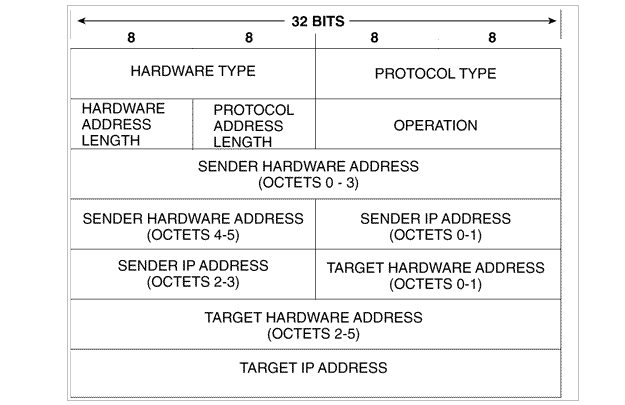
\includegraphics[scale=0.6]{arp.png}\\
\textbf{ARP poisoning}\\
The ARP protocol is declarative, it does not need an answer.\\
Nodes are not authenticated.\\
Limitations: it works only on LAN\\\\
\newpage
\textbf{Subnets and CIDR}\\
Subnets are logical divisions of IP addresses. IP bits are partitioned as network,subnet,host.\\
A subnet mask indicates sections of IP addresses meant for network and subnet.\\
Eg. 255.255.255.0 means 24 bits for network and subnet and 8 bits for hosts.\\\\
\textbf{CIDR}\\
Classless Inter Domain Routing, it is a synthetic way to represent subnet masks.\\
\emph{Example: }
\begin{itemize}
\item Network mask: 255.255.0.0.
\item CIDR representation: 132.132.1.10/16
\item Hosts = $2^{16}$
\end{itemize}
\emph{Formulas:} (everything as binary)
\begin{itemize}
\item Network = Ip AND Subnet
\item Host = Ip AND Not(Subnet)
\end{itemize}
\newpage
\subsection{IP}
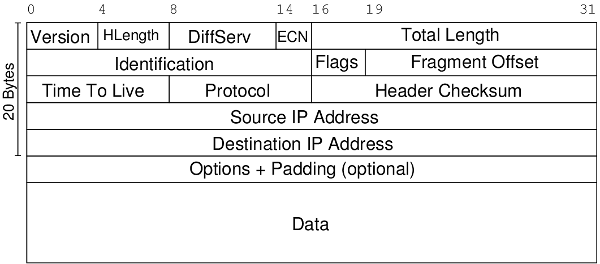
\includegraphics[scale=0.5]{ip.png}\\
Some IPs are reserved for private networks:
\begin{itemize}
\item 10.0.0.0 $\to$ 10.255.255.255
\item 192.168.1.1 $\to$ 192.168.255.255
\item 172.16.0.0 $\to$ 172.16.255.255
\end{itemize}
\textbf{Def} A \emph{datagram} is a basic transfer unit associated with a packet-switched network. The delivery, arrival time, and order of arrival need not be guaranteed by the network.\\\\
\textbf{Def} MTU maximum transmission unit\\\\
\textbf{IP fragmentation}
\emph{Identification:} 16 bit, is the unique identifier of the fragmented datagram.\\
Note that all fragments have the same identification number.\\
\emph{Flags:} 3 bits
\begin{itemize}
\item 0 Reserved, must be zero
\item DF Don't fragment\\
If set to 0 $\to$ there may be fragments\\
If set to 1 $\to$ drop datagram if it has to be fragmented
\item MF More fragments\\
0 $\to$ last fragment\\
1 $\to$ there are more fragments
\end{itemize}
\emph{Offset} 13 bits, offset of this datagram wrt the first fragment with that ID
\newpage
\textbf{Fragmentation example}\\\\
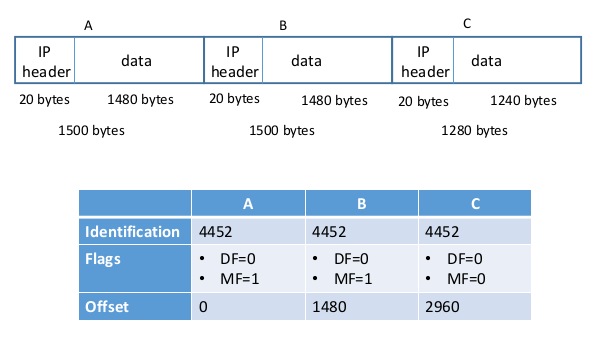
\includegraphics[scale=0.6]{fragmentation.png}\\
\begin{remark}
\textbf{DOS with IP fragments}
You keep sending fragments without sending the first fragment, the router keeps waiting for it until it exhausts its memory.
\end{remark}
\newpage
\subsection{ICMP} Internet control message protocol. It relies on IP and is and integral part of it.\\\\
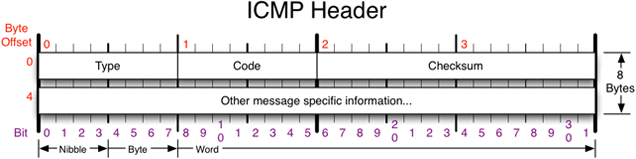
\includegraphics[scale=0.9]{icmp.png}\\\\
\textbf{Some message types}
\begin{itemize}
\item 0		Echo Reply
\item 3		Destination	Unreachable\\
Code 0 $\to$ Net unreachable\\
Code 1 $\to$ Host unreachable\\
Code 2 $\to$ Protocol unreachable\\
Code 3 $\to$ Port unreachable\\
Code 4 $\to$ Fragmentation needed and DF set\\
Code 5 $\to$ Source route failed
\item 4		Source	Quench
\item 5		Redirect
\item 8		Echo
\item 11		Time Exceeded\\
Code 0 $\to$ Net unreachable\\
Code 1 $\to$ Host unreachable
\item 12		Parameter Problem
\item 13		Timestamp
\item 14		Timestamp Reply
\item 15		Information	Request
\item 16		Information	Reply
\end{itemize}
\subsection{Traceroute}
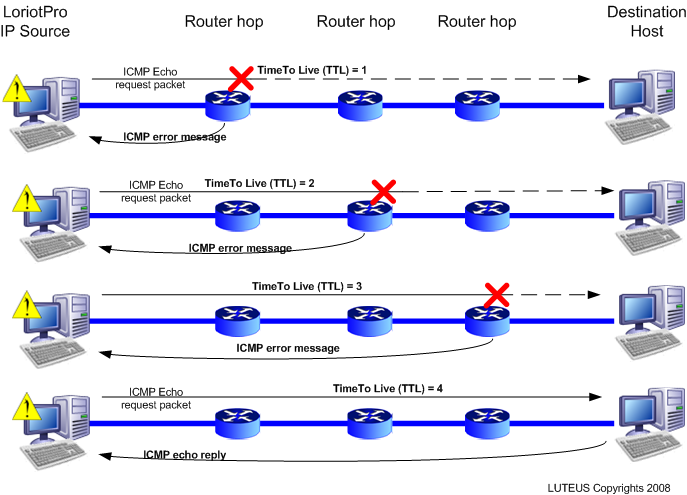
\includegraphics[scale=0.5]{traceroute.png}
\newpage
\subsection{Denial of service}
\textbf{Def} a Denial of Service is a type of attack that aims at congesting or overpowering a system's capacity by generating requests the system will have to answer.\\\\
\textbf{Examples}
\begin{itemize}
\item Dos with IP fragmentation
\item Ping Flooding (the attacker exploit his wider bandwidth)
\item Ping of death
\end{itemize}




\end{document}